\documentclass{../grid-link-report}
\SetClassAssetsDir{../class-assets}

\newcommand{\projectassetsdir}{../project-assets}

\project{Heywood BESS}
\client{Atmos Renewables}
\title{Modelling report - aggregation methodology}
\docnumber{HEYWOODBESS-GR-RPT-005}
\issueddate{24 July 2025}
\revision{1-0-0}
\revisionhistorycsvpath{report-assets/revisionhistory.csv}
\clientlogopath{\projectassetsdir/client-logo.jpg}

\usepackage{listings}
\usepackage{tabto}
\usepackage[justification=centering]{caption}%
\usepackage{pgfplotstable} % For reading and displaying tables from CSV files
\usepackage{booktabs}      % For better-looking tables

\begin{document}
	% Draft commands
	%\adddraftstamp
	%\listoftodos
	
	\frontmatter
	\maketitle  
	
	\makedisclaimer
	\clearpage
	\tableofcontents
	\makerevisionhistorypage
	%\makeaboutgridlink
	
	\mainmatter
	
	\chapter{Introduction}
	This report is intended to summarise the work completed as part of the development of SMIB models for Heywood BESS R0 in PSCAD and PSSE. As such, this report will:
	
	\begin{itemize}
		\item Describe the input data used to model the \acs{BESS}.
		\item Describe the methodology used to create an aggregated or lumped model.
		\item Assess the variation between the lumped models (PSCAD and PSSE) and the disaggregated model (PowerFactory) with respect to the losses in individual elements in each model.
	\end{itemize}

	\chapter{Project overview}
	The Heywood Battery Energy Storage System (HEYWOODBESS) is a $\pm~285MW/1140MWh$ Battery Energy Storage Project, is located 5 km from the town of Heywood and 300 km west of Melbourne in Victoria as shown in Figure~\ref{fig:project-location}. The project is expected to connect directly to the existing 275 kV Heywood terminal station via a single high voltage cable.

HEYWOODBESS will include 92 SMA Sunny Central 4.6 MVA (SCS 4600 UP-S) converters which will be connected to two 275/33/33kV, 160MVA three winding transformers through a 33kV reticulation system. Each converter will have a dedicated 33/0.69kV, 4.6 MVA step up transformer.


\begin{figure}[H]
	\centering
	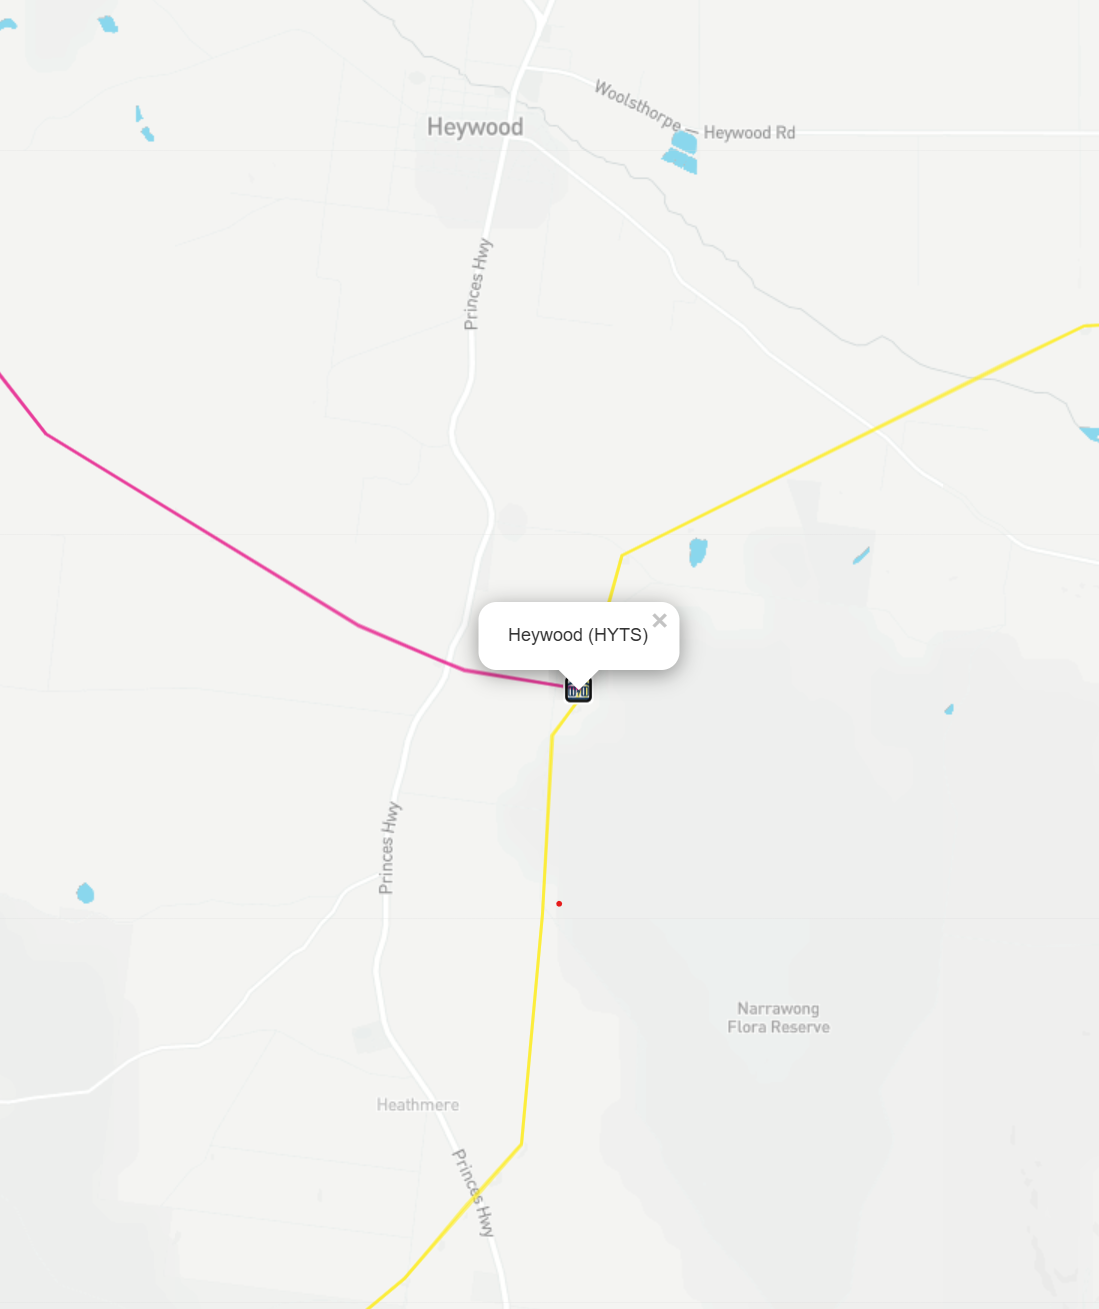
\includegraphics[width=0.7\textwidth]{\projectassetsdir/project-location.png} % Change example-image-a to the filename of your image
	\caption{Project location}
	\label{fig:project-location}
\end{figure}



	\chapter{Input data}
	\label{Input Data}
	\section{Grid transformers}
	
	This project is at R0 stage, and therefore design parameters for equipment are not yet final. Early stage design works have been used to derive parameters for use in power system models. The two 275/33/33 kV grid transformers have been modelled in all power system models used, with no aggregation. The following parameters, as entered into the PSCAD model in Table \ref{tab:aggr-transformer}, apply to the main grid transformers.
	
			% Aggregate transformer parameter table
	{%
		\thicktablelines
		\begin{longtable}{|C{6cm}|C{6cm}|} 
			\caption{Grid transformer parameters}
			\label{tab:aggr-transformer}
			\\	
			\toprule
			
			\rowcolor{tableheaderblue}
			\bfseries \color{white}Parameter & \bfseries \color{white}Value
			\endhead
			\bottomrule \endfoot
			\csvreader[
			separator=comma,
			late after line=\\\hline,
			late after last line=,
			before reading={\catcode`\#=12},
			after reading={\catcode`\#=6}]%
			{report-assets/GTX.csv}{1=\COLA,2=\COLB}{\COLA & \COLB}
			\\\hline
		\end{longtable}
	}

	
	\section{Medium voltage transformers}


    Preliminary input parameters for the 4.6 MVA medium voltage converter transformers were provided by BEE as part of their initial design. These parameters align with the range of allowed impedances specified in SMA's Grid Modelling Guidelines for converter transformers. Parameters for an individual transformer, as entered into PSCAD, before scaling was applied, is shown in Table \ref{tab:inv-transformer}. 
    
    Scaling in PSCAD was applied via a current scaling element, with 4 groups of 23 transformers modelled. In PSSE, scaling was applied manually to the MVA base of the transformer for aggregation purposes, and to non per unit parameters, such as copper losses.

	{%
		\thicktablelines
		\begin{longtable}{|C{6cm}|C{6cm}|} 
			\caption{Converter transformer parameters}
			\label{tab:inv-transformer}
			\\	
			\toprule
			
			\rowcolor{tableheaderblue}
			\bfseries \color{white}Parameter & \bfseries \color{white}Value
			\endhead
			\bottomrule \endfoot
			\csvreader[
			separator=comma,
			late after line=\\\hline,
			late after last line=,
			before reading={\catcode`\#=12},
			after reading={\catcode`\#=6}]%
			{report-assets/INVTX.csv}{1=\COLA,2=\COLB}{\COLA & \COLB}
			\\\hline
		\end{longtable}
	}
	
	\section{MV reticulation}
	The cable lengths and cable types for the BESS medium voltage reticulation network were aggregated from the input cable schedule.\cite{MV cable schedule} The cable schedule was directly replicated in the BESS PowerFactory model also provided as an input to the grid studies by the electrical design consultant. 
	
	A visual representation of the preliminary electrical arrangement of the BESS has been provided in Figure \ref{fig:mv_sld1-2} below, which shows the layout of 33 kV switchboards 1 and 2, which connect to the two 33 kV windings of one of the grid transformers. Switchboards 3 and 4, not shown here, have a similar configuration.
	
	\begin{figure}[h]
		\centering
		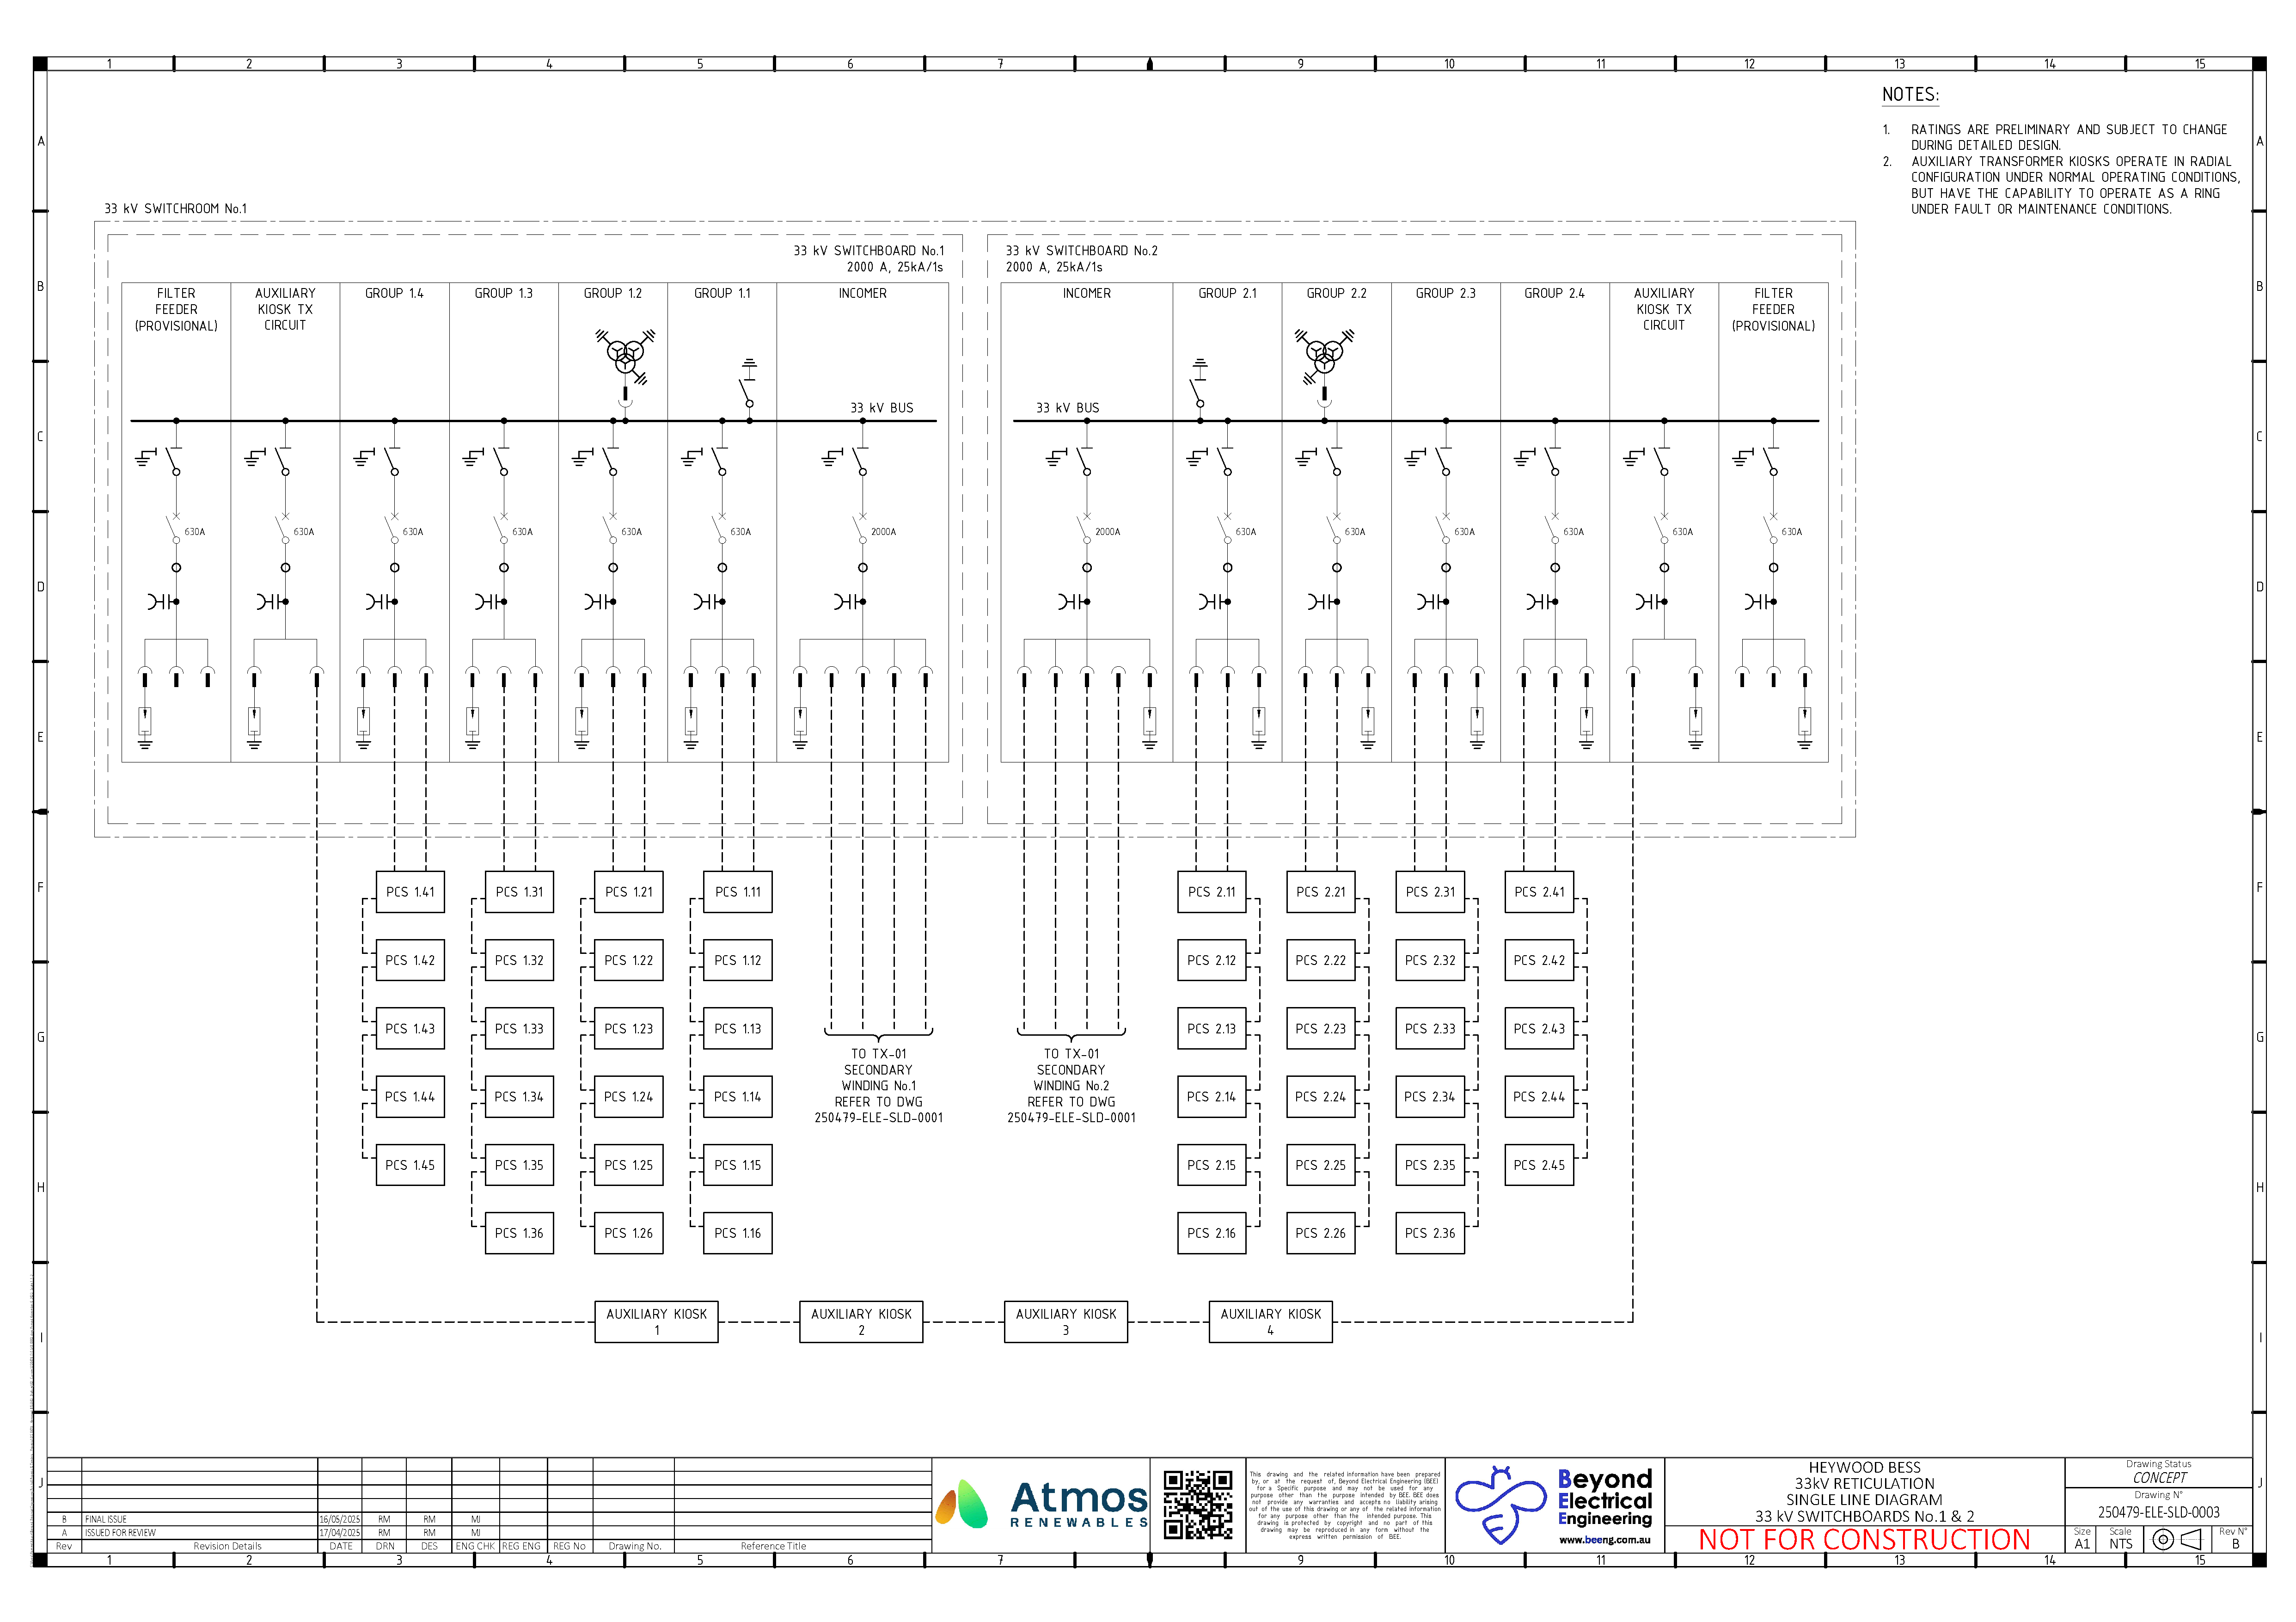
\includegraphics[width=1.0\textwidth]{report-assets/images/250479-ELE-SLD-0003_B_33kV Reticulation SLD SB1-2.pdf}
		\caption{MV single line diagram - switchboard 1 and 2}
		\label{fig:mv_sld1-2}
	\end{figure}	

	\chapter{Aggregation methodology}
	
	\section{Aggregation of each feeder}
	\label{Aggregation Of Each Feeder}
	The lumped model of the BESS was developed with the inputs provided in section \ref{Input Data} and in conjunction with the methodology outlined in the NREL paper "Equivalencing the Collector System of a Large Wind Power Plant".\cite{equivalence paper 2006}.
	
	This technical paper outlines that each daisy-chained feeder (a) has an equivalent representation as pictured in (b).
	
	\begin{figure}[h]
		\centering
		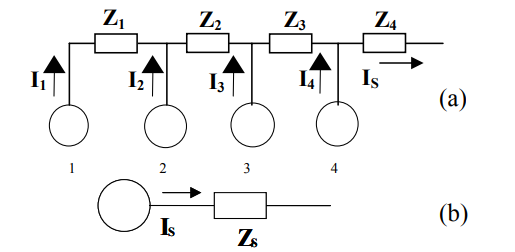
\includegraphics[width=0.6\textwidth]{report-assets/images/feeder_equivalence.png}
		\caption{Feeder equivalent circuit}
		\label{fig:feeder_equivalance}
	\end{figure}	
	
	Defining this equivalent circuit allows the total impedance for the feeder to be written as follows.
	
	\begin{equation}
		Z_{s} = \frac{\sum_{m=1}^{n}m^{2}Z_{m}}{n^2}
	\end{equation}
	
	where $Z_{m}$ represents the individual series impedances.
	
	This method of impedance aggregation was applied in calculating equivalent positive and zero sequence resistance, reactance and susceptance parameters for each feeder.
	 
	\section{Aggregation up to the 33kV bus}
	\label{Aggregation Up to the 33kV Bus}	

	After calculating the aggregated impedance for each feeder, an equivalent circuit of each 33kV bus can be represented as per the below Figure \ref{fig:bus_equivalance}.
	
	\begin{figure}[H]
		\centering
		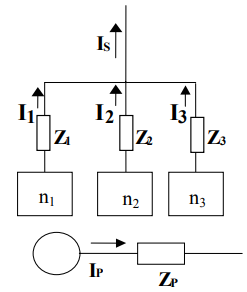
\includegraphics[width=0.3\textwidth]{report-assets/images/bus_equivalence.png}
		\caption{33kV bus equivalent circuit}
		\label{fig:bus_equivalance}
	\end{figure}	
	
	Defining this equivalent circuit allows the total impedance of each 33kV bus to be written as follows
	\begin{equation}
		Z_{p} = \frac{\sum_{m=1}^{n}n_{m}^{2}Z_{m}}
					 {[\sum_{m=1}^{n}n_{m}]^2}
	\end{equation}
	
	where Zm represents the equivalent impedance of the individual parallel groups. 
	
	\section{Aggregation up to each main transformer}	
	Once reticulation impedances were aggregated up to each 33kV bus (as per Section \ref{Aggregation Up to the 33kV Bus}), these were applied to two impedance elements in PSCAD and PSSE models. This results in the formulation of the aggregated or lumped impedance between the MV windings of the 3 winding grid transformer and the aggregated unit transformers.
	
	This impedance was then utilised in preparing the plants PSCAD and PSSE \ac{SMIB} models.

	\chapter{Model benchmarking}
	
	\section{Powerfactory model}
	The PowerFactory model for \project ~ is shown in Figures \ref{fig:powerfactory_model} and \ref{fig:powerfactory_model_33_SB} below. 
	
	The PowerFactory model was initially developed by BEE based on their preliminary design. It was modified by Grid-Link to incorporate AusNet's estimated parameters for the 1.4 km, 275 kV high-voltage cable between the Heywood terminal station and the substation. 
	
	Figure \ref{fig:powerfactory_model_33_SB} shows 33 kV switchboard 1 - which connects to feeders 1.1-1.4. Each feeder has either five or six 4.6 MVA power conversion stations, with 23x 4.6 MVA power conversion stations in total.
	
	Similarly, 33 kV switchboards 2-4 each have 23x 4.6 MVA power conversion stations connected via four feeders.
	
	\begin{figure}[H]
		\centering
		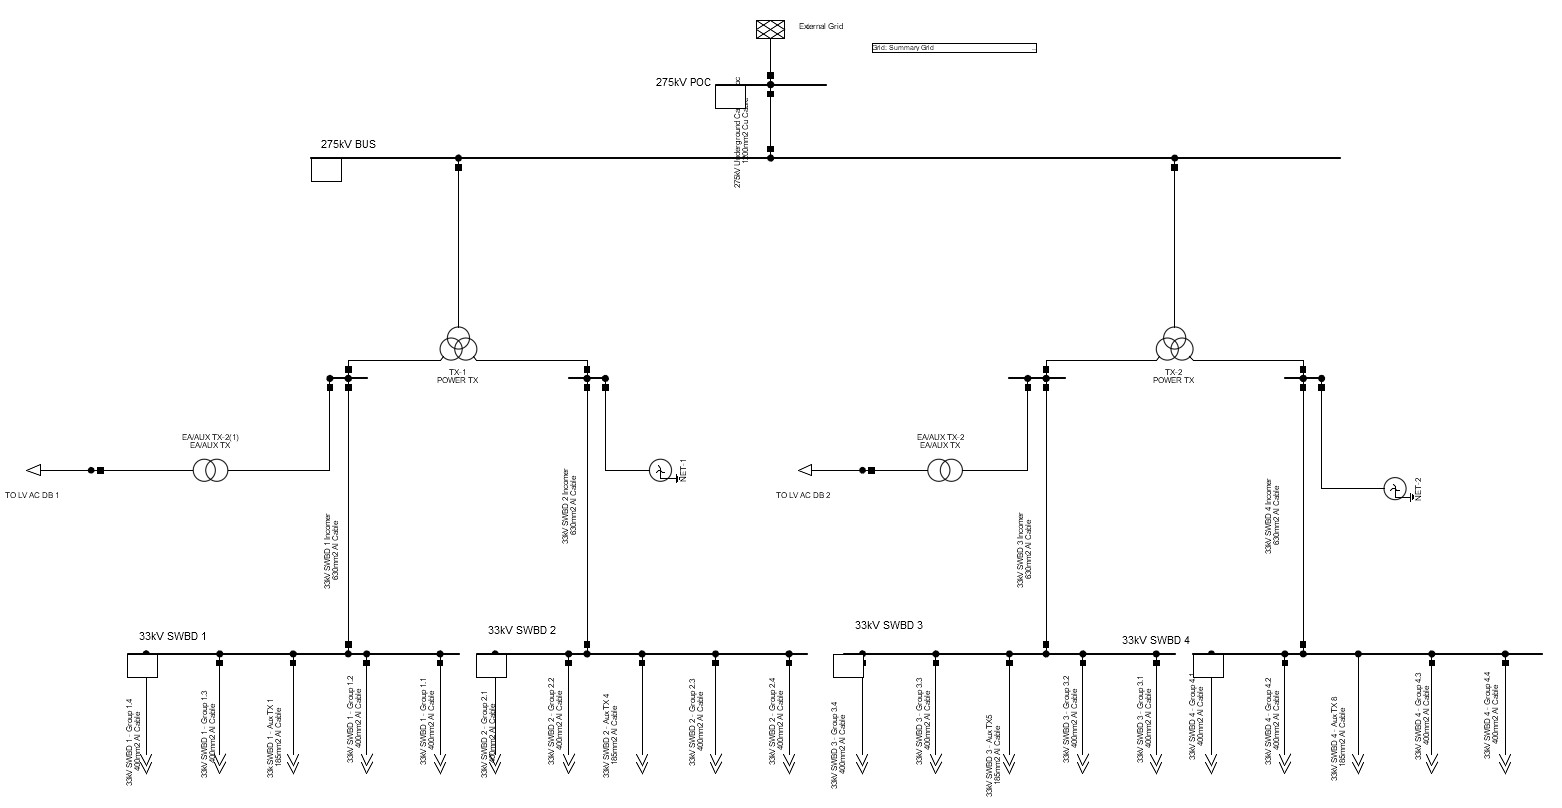
\includegraphics[width=0.9\textwidth]{report-assets/images/pf-screenshot.jpg}
		\caption{Powerfactory Model Grid Connection}
		\label{fig:powerfactory_model}
	\end{figure}
	
	\begin{figure}[H]
		\centering
		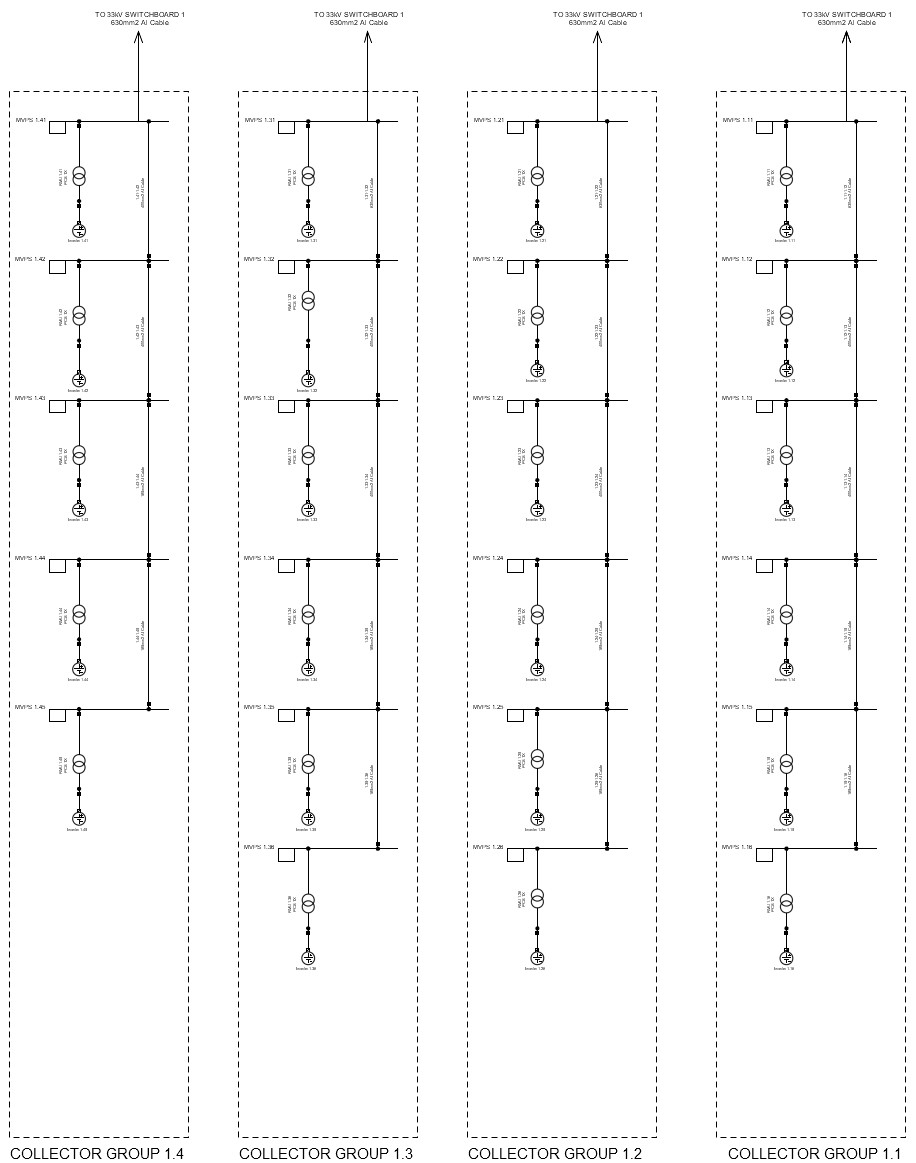
\includegraphics[width=0.8\textwidth]{report-assets/images/pf-screenshot-33.jpg}
		\caption{Powerfactory Model 33 kV Switchboard 1}
		\label{fig:powerfactory_model_33_SB}
	\end{figure}
	
	\section{PSCAD model}
	The aggregated PSCAD model for \project ~ is shown in Figure \ref{fig:pscad_model}. 
	
	Each branch to the left of the grid transformers is composed of 23 equivalent SCS 4600 UP-S converters - each complete with its own 4.6 MVA medium voltage transformer. 
	
	The PI sections to the right of each main unit transformer incorporate the associated aggregated medium voltage impedance of the cable reticulation network. Each feeder is represented by two lumped impedance elements, which represent the daisy chained feeders, and the impedance between the 33 kV bus and the grid transformer respectively.

	
	\begin{figure}[H]
		\centering
		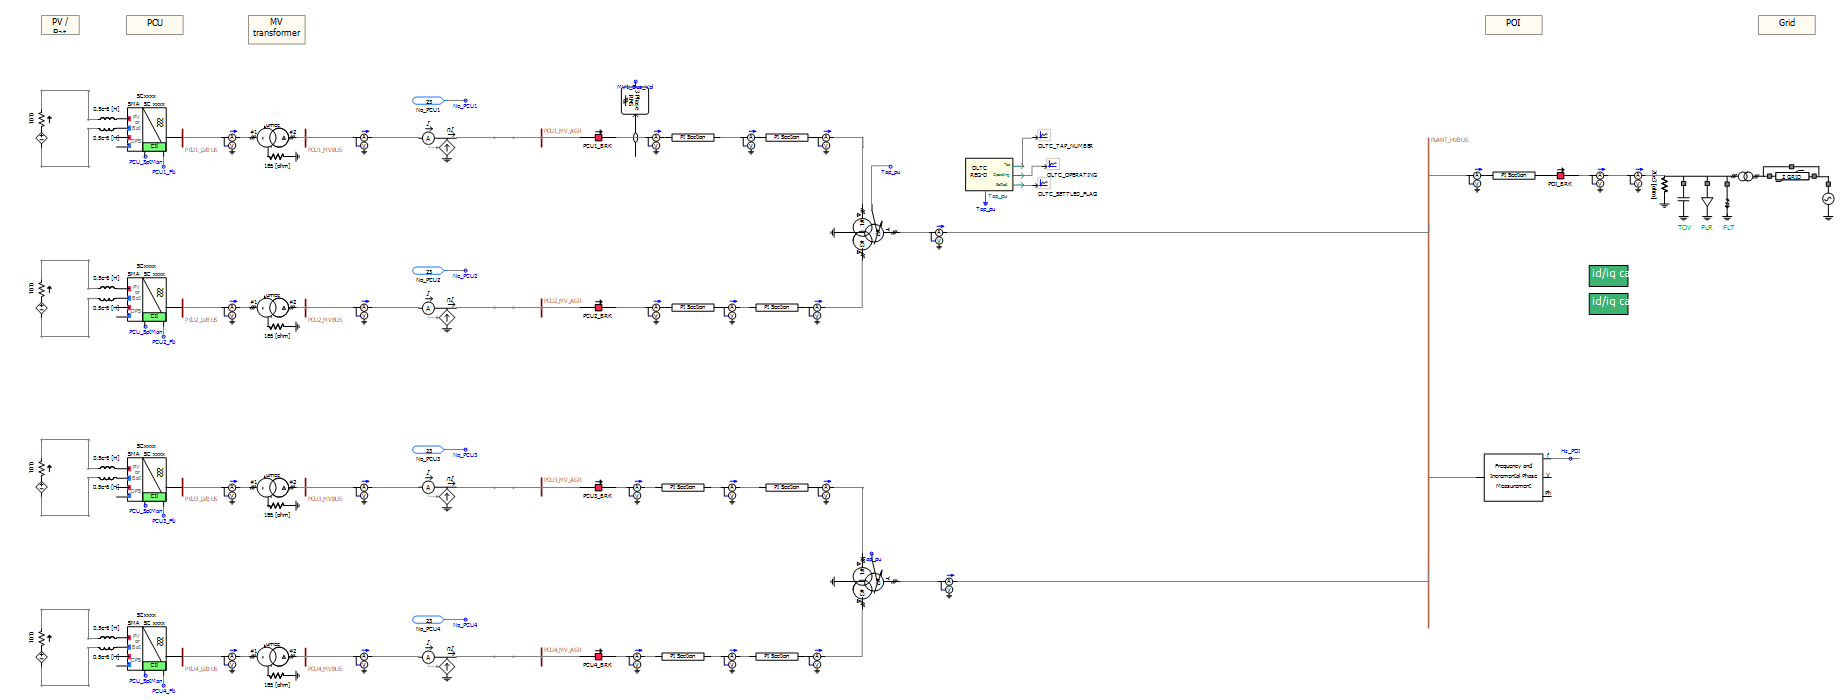
\includegraphics[width=1.0\textwidth]{report-assets/images/pscad-model-screenshot.png}
		\caption{Aggregated PSCAD Model}
		\label{fig:pscad_model}
	\end{figure}	
	
	\section{PSSE model}
	The aggregated PSSE model for \project ~ is shown in Figure \ref{fig:psse_model}. 
	
	Each branch to the left of the grid transformers is composed of 23 equivalent SCS 4600 UP-S converters - each complete with its own 4.6 MVA medium voltage transformer, scaled up by a factor of 23.
	
	The line sections to the right of each main unit transformer incorporate the associated aggregated medium voltage impedance of the cable reticulation network. As per PSCAD, each feeder is represented by two lumped impedance elements, which represent the daisy chained feeders, and the impedance between the 33 kV bus and the grid transformer respectively.
	
	\begin{figure}[H]
		\centering
		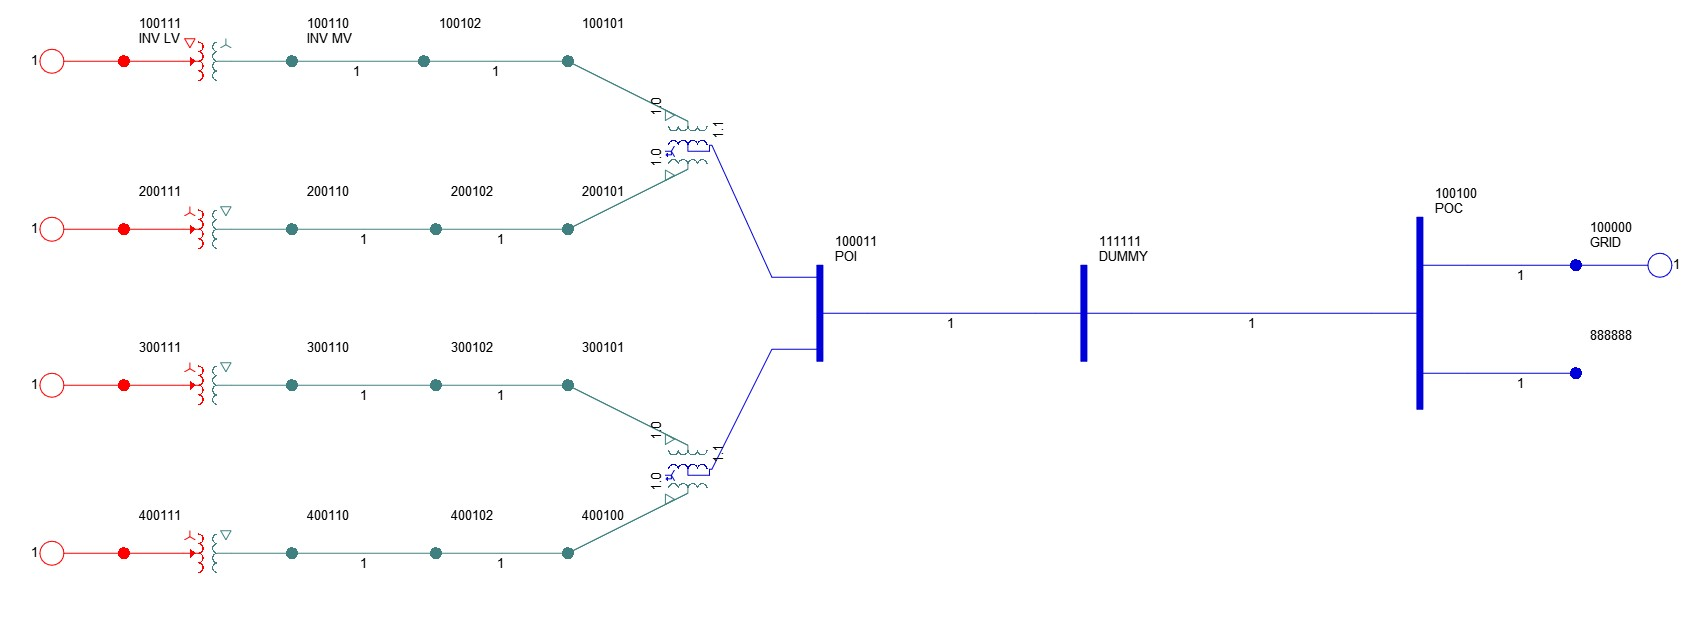
\includegraphics[width=1\textwidth]{report-assets/images/psse-screenshot.jpg}
		\caption{Aggregated PSSE Model}
		\label{fig:psse_model}
	\end{figure}
	
	
	\section{Analysis and results}
	
	To determine the validity of the aggregated model, the variation between each lumped model and the disaggregated PowerFactory model was compared. Specifically, the variation between active and reactive power losses across the 220/33/33kV transformers, the 33kV reticulation network and the 33/0.69kV transformers was compared between both models for the below operating points. These operating points represent the 'corner points' of the plant capability under steady state conditions and Vpoc is the expected normal operating voltage at the point of connection.

	\begin{enumerate}
		\item $P_{poc}$ = 285 MW, $Q_{poc}$ = 112.575 MVAr, $V_{poc}$ = 1.06 pu
		\item $P_{poc}$ = 285 MW, $Q_{poc}$ = -112.575 MVAr, $V_{poc}$ = 1.06 pu
		\item $P_{poc}$ = 285 MW, $Q_{poc}$ =  0.0MVAr, $V_{poc}$ = 1.06 pu
		\item $P_{poc}$ = 0 MW, $Q_{poc}$ = 112.575 MVAr, $V_{poc}$ = 1.06 pu
		\item $P_{poc}$ = 0 MW, $Q_{poc}$ = -112.575 MVAr, $V_{poc}$ = 1.06 pu
		\item $P_{poc}$ = 0 MW, $Q_{poc}$ =  0.0MVAr, $V_{poc}$ = 1.06 pu
		\item $P_{poc}$ = -285 MW, $Q_{poc}$ = 112.575 MVAr, $V_{poc}$ = 1.06 pu
		\item $P_{poc}$ = -285 MW, $Q_{poc}$ = -112.575 MVAr, $V_{poc}$ = 1.06 pu
		\item $P_{poc}$ = -285 MW, $Q_{poc}$ =  0.0MVAr, $V_{poc}$ = 1.06 pu
	\end{enumerate}
	
	A load flow was performed on the PowerFactory model platform at the above operating points to collect losses data for each component. The voltage, active power and reactive power at the point of connection was compared across all platforms to ensure the models were aligned. The PSCAD model was initialised as close as practicably possible to these setpoints and data was collected for a flat run to compare the two models. A load flow was also performed on the PSSE model at the setpoints described, to collect losses data.
	
	\subsubsection{Reticulation Losses}
	\label{Reticulation mismatch}
	For each model, the difference between the aggregate active and reactive power leaving the \ac{HV} winding(s) of the converter transformers and the power flowing into the \ac{LV} winding(s) of the grid transformers was determined to establish losses in the reticulation network.
	
	1. Using the PowerFactory model the total active and reactive consumption across each cable segment in the 33kV reticulation network was extracted from the flexible data table and summated.
	
	2. To get the same quantities in PSCAD, the active and reactive power flows were monitored on either side of the two lumped PI sections representing the 33kV reticulation network, which were then compared to derive the losses across all 33kV cables.
	
	3. The losses were extracted from the PSSE model by subtracting the measured flow into the grid transformer from the flow out of the converter transformer. The values for each lumped section were then compared to derive the losses across all 33kV cables.
	
	Losses in each model were then compared. The difference or delta between each models losses has been used as a point of comparison to establish that the aggregation methodology used for the MV reticulation network is fit for purpose.
	
	The mismatch in active and reactive power through the \ac{MV} reticulation was compared between both models and summarised in \ref{tab:reticulation_results_pscad} and \ref{tab:reticulation_results_psse}. 
	
	\begin{itemize}
		\item The largest absolute mismatch in active power was 0.009 MW across all scenarios.
		\item The largest absolute mismatch in reactive power was 0.058 MVAr across all scenarios.
	\end{itemize} 
	
	{%
		\thicktablelines
		\begin{longtable}{|C{1.7cm}|C{1.5cm}|C{1.7cm}|C{1.5cm}|C{1.5cm}|C{1.5cm}|C{1.5cm}|C{1.5cm}|C{1.5cm}|} 
			\caption{Reticulation results - Powerfactory vs PSCAD}
			\label{tab:reticulation_results_pscad}
			\\	
			\toprule
			\rowcolor{tableheaderblue}
			\multicolumn{3}{c|}{\bfseries \color{white}\rule{0pt}{1.5em}} & \multicolumn{2}{c|}{\bfseries \color{white}Powerfactory} & \multicolumn{2}{c|}{\bfseries \color{white}PSCAD} & \multicolumn{2}{c|}{\bfseries \color{white}Delta}\\
			\hline
			\rowcolor{tableheaderblue}
			\bfseries \color{white}Test Number & \bfseries \color{white}P_POC (MW) & \bfseries \color{white}Q_POC (MVAr) & \bfseries \color{white}dP (MW) & \bfseries \color{white}dQ (MVAr) & \bfseries \color{white}dP (MW) & \bfseries \color{white}dQ (MVAr) & \bfseries \color{white}dP (MW) & \bfseries \color{white}dQ (MVAr)\\
			\endhead
			
			\bottomrule \endfoot
			\csvreader[
			separator=comma,
			late after line=\\\hline,
			late after last line=,
			before reading={\catcode`\#=12},
			after reading={\catcode`\#=6}]%
			{report-assets/Reticulation losses pf vs pscad.csv}{1=\COLA,2=\COLB,3=\COLC,4=\COLD,5=\COLE,6=\COLF,7=\COLG,8=\COLH,9=\COLI}{\COLA & \COLB & \COLC & \COLD & \COLE & \COLF & \COLG & \COLH & \COLI}
			\\\hline
		\end{longtable}
	}
	
	{%
		\thicktablelines
		\begin{longtable}{|C{1.7cm}|C{1.5cm}|C{1.7cm}|C{1.5cm}|C{1.5cm}|C{1.5cm}|C{1.5cm}|C{1.5cm}|C{1.5cm}|} 
			\caption{Reticulation results - Powerfactory vs PSSE}
			\label{tab:reticulation_results_psse}
			\\	
			\toprule
			\rowcolor{tableheaderblue}
			\multicolumn{3}{c|}{\bfseries \color{white}\rule{0pt}{1.5em}} & \multicolumn{2}{c|}{\bfseries \color{white}Powerfactory} & \multicolumn{2}{c|}{\bfseries \color{white}PSSE} & \multicolumn{2}{c|}{\bfseries \color{white}Delta}\\
			\hline
			\rowcolor{tableheaderblue}
			\bfseries \color{white}Test Number & \bfseries \color{white}P_POC (MW) & \bfseries \color{white}Q_POC (MVAr) & \bfseries \color{white}dP (MW) & \bfseries \color{white}dQ (MVAr) & \bfseries \color{white}dP (MW) & \bfseries \color{white}dQ (MVAr) & \bfseries \color{white}dP (MW) & \bfseries \color{white}dQ (MVAr)\\
			\endhead
			
			\bottomrule \endfoot
			\csvreader[
			separator=comma,
			late after line=\\\hline,
			late after last line=,
			before reading={\catcode`\#=12},
			after reading={\catcode`\#=6}]%
			{report-assets/Reticulation losses pf vs psse.csv}{1=\COLA,2=\COLB,3=\COLC,4=\COLD,5=\COLE,6=\COLF,7=\COLG,8=\COLH,9=\COLI}{\COLA & \COLB & \COLC & \COLD & \COLE & \COLF & \COLG & \COLH & \COLI}
			\\\hline
		\end{longtable}
	}
	
	To review the full output of results please refer to appendix A.
	
	\subsubsection{Transformer mismatch}
	\label{Transformer mismatch}
	The power flow entering the LV winding(s) of any given transformer was compared with the power flow leaving its HV winding.
	
	1. Using the PowerFactory model the total active and reactive consumption across each transformer was extracted from the flexible data table and a summation was made for the main transformers and for the converter transformers independently.
	
	2. To get the same quantities in PSCAD and PSSE, the active and reactive power flows were monitored on either side of the four aggregated medium voltage transformers as well as for the two main transformers.
	
	Losses in each model were then compared. The difference or delta between each models losses has been used as a point of comparison to establish that the aggregation methodology used for the converter transformers is fit for purpose, and that the grid transformer parameters have been accurately translated between models.
	
	These model discrepancies were then averaged across all transformers to represent the mismatch per transformer. 
	
	From the table below we make the following observations
	\begin{itemize}
		\item For the converter transformers we see that the largest total active power mismatch between models was  0.038 MW, while the largest total reactive power mismatch was 0.767 MVAr.
		\item For the grid transformers we see that the largest total active power mismatch between models was 0.023 MW, while the largest total reactive power mismatch between models was 0.965 MVAr.
		
	\end{itemize} 
	
	{%
		\thicktablelines
		\begin{longtable}{|C{1.7cm}|C{1.5cm}|C{1.7cm}|C{1.5cm}|C{1.5cm}|C{1.5cm}|C{1.5cm}|C{1.5cm}|C{1.5cm}|} 
			\caption{Converter transformer results - Powerfactory vs PSCAD}
			\label{tab:unit_TX_results_pscad}
			\\	
			\toprule
			\rowcolor{tableheaderblue}
			\multicolumn{3}{c|}{\bfseries \color{white}\rule{0pt}{1.5em}} & \multicolumn{2}{c|}{\bfseries \color{white}Powerfactory} & \multicolumn{2}{c|}{\bfseries \color{white}PSCAD} & \multicolumn{2}{c|}{\bfseries \color{white}Delta}\\
			\hline
			\rowcolor{tableheaderblue}
			\bfseries \color{white}Test Number & \bfseries \color{white}P_POC (MW) & \bfseries \color{white}Q_POC (MVAr) & \bfseries \color{white}dP (MW) & \bfseries \color{white}dQ (MVAr) & \bfseries \color{white}dP (MW) & \bfseries \color{white}dQ (MVAr) & \bfseries \color{white}dP (MW) & \bfseries \color{white}dQ (MVAr)\\
			\endhead
			
			\bottomrule \endfoot
			\csvreader[
			separator=comma,
			late after line=\\\hline,
			late after last line=,
			before reading={\catcode`\#=12},
			after reading={\catcode`\#=6}]%
			{report-assets/Unit TX losses PSCAD.csv}{1=\COLA,2=\COLB,3=\COLC,4=\COLD,5=\COLE,6=\COLF,7=\COLG,8=\COLH,9=\COLI}{\COLA & \COLB & \COLC & \COLD & \COLE & \COLF & \COLG & \COLH & \COLI}
			\\\hline
		\end{longtable}
	}
	
	{%
		\thicktablelines
		\begin{longtable}{|C{1.7cm}|C{1.5cm}|C{1.7cm}|C{1.5cm}|C{1.5cm}|C{1.5cm}|C{1.5cm}|C{1.5cm}|C{1.5cm}|} 
			\caption{Unit transformer results - Powerfactory vs PSSE}
			\label{tab:unit_TX_results_psse}
			\\	
			\toprule
			\rowcolor{tableheaderblue}
			\multicolumn{3}{c|}{\bfseries \color{white}\rule{0pt}{1.5em}} & \multicolumn{2}{c|}{\bfseries \color{white}Powerfactory} & \multicolumn{2}{c|}{\bfseries \color{white}PSSE} & \multicolumn{2}{c|}{\bfseries \color{white}Delta}\\
			\hline
			\rowcolor{tableheaderblue}
			\bfseries \color{white}Test Number & \bfseries \color{white}P_POC (MW) & \bfseries \color{white}Q_POC (MVAr) & \bfseries \color{white}dP (MW) & \bfseries \color{white}dQ (MVAr) & \bfseries \color{white}dP (MW) & \bfseries \color{white}dQ (MVAr) & \bfseries \color{white}dP (MW) & \bfseries \color{white}dQ (MVAr)\\
			\endhead
			
			\bottomrule \endfoot
			\csvreader[
			separator=comma,
			late after line=\\\hline,
			late after last line=,
			before reading={\catcode`\#=12},
			after reading={\catcode`\#=6}]%
			{report-assets/Unit TX losses PSSE.csv}{1=\COLA,2=\COLB,3=\COLC,4=\COLD,5=\COLE,6=\COLF,7=\COLG,8=\COLH,9=\COLI}{\COLA & \COLB & \COLC & \COLD & \COLE & \COLF & \COLG & \COLH & \COLI}
			\\\hline
		\end{longtable}
	}
	
	{%
		\thicktablelines
		\begin{longtable}{|C{1.7cm}|C{1.5cm}|C{1.7cm}|C{1.5cm}|C{1.5cm}|C{1.5cm}|C{1.5cm}|C{1.5cm}|C{1.5cm}|} 
			\caption{Grid transformer results - Powerfactory vs PSCAD}
			\label{tab:grid_TX_results_pscad}
			\\	
			\toprule
			\rowcolor{tableheaderblue}
			\multicolumn{3}{c|}{\bfseries \color{white}\rule{0pt}{1.5em}} & \multicolumn{2}{c|}{\bfseries \color{white}Powerfactory} & \multicolumn{2}{c|}{\bfseries \color{white}PSCAD} & \multicolumn{2}{c|}{\bfseries \color{white}Delta}\\
			\hline
			\rowcolor{tableheaderblue}
			\bfseries \color{white}Test Number & \bfseries \color{white}P_POC (MW) & \bfseries \color{white}Q_POC (MVAr) & \bfseries \color{white}dP (MW) & \bfseries \color{white}dQ (MVAr) & \bfseries \color{white}dP (MW) & \bfseries \color{white}dQ (MVAr) & \bfseries \color{white}dP (MW) & \bfseries \color{white}dQ (MVAr)\\
			\endhead
			
			\bottomrule \endfoot
			\csvreader[
			separator=comma,
			late after line=\\\hline,
			late after last line=,
			before reading={\catcode`\#=12},
			after reading={\catcode`\#=6}]%
			{report-assets/Grid TX losses PSCAD.csv}{1=\COLA,2=\COLB,3=\COLC,4=\COLD,5=\COLE,6=\COLF,7=\COLG,8=\COLH,9=\COLI}{\COLA & \COLB & \COLC & \COLD & \COLE & \COLF & \COLG & \COLH & \COLI}
			\\\hline
		\end{longtable}
	}
	
	{%
		\thicktablelines
		\begin{longtable}{|C{1.7cm}|C{1.5cm}|C{1.7cm}|C{1.5cm}|C{1.5cm}|C{1.5cm}|C{1.5cm}|C{1.5cm}|C{1.5cm}|} 
			\caption{Grid transformer results - Powerfactory vs PSSE}
			\label{tab:grid_TX_results_psse}
			\\	
			\toprule
			\rowcolor{tableheaderblue}
			\multicolumn{3}{c|}{\bfseries \color{white}\rule{0pt}{1.5em}} & \multicolumn{2}{c|}{\bfseries \color{white}Powerfactory} & \multicolumn{2}{c|}{\bfseries \color{white}PSSE} & \multicolumn{2}{c|}{\bfseries \color{white}Delta}\\
			\hline
			\rowcolor{tableheaderblue}
			\bfseries \color{white}Test Number & \bfseries \color{white}P_POC (MW) & \bfseries \color{white}Q_POC (MVAr) & \bfseries \color{white}dP (MW) & \bfseries \color{white}dQ (MVAr) & \bfseries \color{white}dP (MW) & \bfseries \color{white}dQ (MVAr) & \bfseries \color{white}dP (MW) & \bfseries \color{white}dQ (MVAr)\\
			\endhead
			
			\bottomrule \endfoot
			\csvreader[
			separator=comma,
			late after line=\\\hline,
			late after last line=,
			before reading={\catcode`\#=12},
			after reading={\catcode`\#=6}]%
			{report-assets/Grid TX losses PSSE.csv}{1=\COLA,2=\COLB,3=\COLC,4=\COLD,5=\COLE,6=\COLF,7=\COLG,8=\COLH,9=\COLI}{\COLA & \COLB & \COLC & \COLD & \COLE & \COLF & \COLG & \COLH & \COLI}
			\\\hline
		\end{longtable}
	}
	
	\subsubsection{HV cable mismatch}
	
	No aggregation was required for the HV cable modelled at 275 kV between the plant and the point of connection at Heywood Terminal station. Differences in losses have been compared in the appendices of this report, but are not material and therefore have not been discussed in detail in this report.
	
	To review the full output of results please refer to the appendix A.
	
	
	\section{Discussion}
	
	As outlined in section \ref{Reticulation mismatch}, the active and reactive power mismatch models for various operating points was not material. An extremely low mismatch was achieved for all elements, with the difference in losses between models equivalent to less than 0.5\% of plant rating.
	
	This suggests that the lumped models (PSCAD and PSSE) are good representations of the disaggregated model (PowerFactory), and that the aggregation methodology used is appropriate for accurate SMIB modelling. 
	
	\chapter*{Acronyms}
\begin{acronym}%[JSONP]\itemsep0pt
	\acro{AAS}{Automatic Access Standard}
	\acro{AEMO}{Australian Energy Market Operator}
	\acro{VSL}{Voltage Stackable Logic}
	\acro{AGC}{Automatic Generation Control}
	\acro{AVR}{Automatic Voltage Regulator}
	\acro{BESS}{Battery Energy Storage System}
	\acro{BOP}{Balance Of Plant}
	\acro{CGBESS}{Clements Gap BESS}
	\acro{Heywood BESS}{Heywood Battery Energy Storage System}	
	\acro{CSR}{Connection Studies Report}
	\acro{CT}{Current Transformer}
	\acro{CUO}{Continuous Uninterrupted Operation}
	\acro{HV}{High Voltage}
	\acro{DMAT}{Dynamic Model Acceptance Test}
	\acro{DYR}{PSSE Dynamics Data File}
	\acro{EMT}{Electromagnetic Transients}
	\acro{FIA}{Full Impact Assessment}
	\acro{FRT}{Fault Ride-Through}
	\acro{GPS}{Generator Performance Standards}
	\acro{HVRT}{High Voltage Ride-Through}
	\acro{LV}{Low Voltage}
	\acro{LVRT}{Low Voltage Ride-Through}
	\acro{MV}{Medium Voltage}
	\acro{NEM}{National Electricity Market}
	\acro{NSP}{Network Service Provider}
	\acro{OEM}{Original Equipment Manufacturer}
	\acro{OFRT}{Over-Frequency Ride-Through}
	\acro{OLTC}{On-Load Tap Changer}
	\acro{OPDMS}{Operations and Planning Data Management System}
	\acro{OVRT}{Over-Voltage Ride-Through}
	\acro{PLL}{Phase-Locked Loop}
	\acro{PLR}{Partial Load Rejection}
	\acro{PPC}{Power Plant Controller}
	\acro{PPM}{Power Plant Manager}
	\acro{RoCoF}{Rate of Change of Frequency}
	\acro{RMS}{Root Mean Square}
	\acro{RMU}{Ring Main Unit}
	\acro{RUG}{Releasable User Guide}
	\acro{S5251}{Reactive Power Capability}
	\acro{S5254}{Generating System Response to Voltage Disturbances}
	\acro{SCR}{Short Circuit Ratio}
	\acro{SMIB}{Single Machine, Infinite Bus}
	\acro{SLD}{Single Line Diagram}
	\acro{TOV}{Temporary Over-Voltage}
	\acro{UFRT}{Under-Frequency Ride-Through}
	\acro{UVRT}{Under-Voltage Ride-Through}
	\acro{VCS}{Voltage Control Strategy}
	\acro{WAN}{Wide Area Network}
	\acro{WF}{Wind Farm}
	\acro{VOIP}{Voice Over Internet Protocol}
	\acro{VRR}{Voltage Regulation Relay}
	\acro{VT}{Voltage Transformer}
\end{acronym}
	\renewcommand\bibname{References}

\begin{thebibliography}{99}	
	\bibitem{mvps-sld}MVPS SLD\\
	(PSD1834-110-001-002.pdf)
	\bibitem{mvt-datasheet}Medium Voltage Transformer Datasheet\\
	(CG_D_00181175_03_General MVT Datasheet.pdf.pdf)
	\bibitem{main-tx-datasheet} Main Transformer Datasheet\\
	(Main Transformer Datasheet.pdf)
	\bibitem{substation-sld} Substation SLD\\
	(PSD1834-110-001-001.pdf)
	\bibitem{avr-manual}TAPCON 230 AVR manual\\
	(bal_3552133_02_001_1_en.pdf)
	\bibitem{oltc-switching} OLTC Switching Datasheet\\
	(VACUTAP®_VV®_Operating_Instructions.pdf)
	\bibitem{harmonic-assessment} Harmonic Emmissions Report\\
	(PSD1834-100-100---Harmonic-Emissions-Assessment-and-Filter-Design-Rev-B.pdf)
	\bibitem{scada-philo} SCADA Control Philosophy\\
	(PSD1834-200-009---SCADA-CONTROL-PHILOSOPHY-Rev.3.pdf)
	\bibitem{aemo-io} AEMO IO Schedule\\
	(PSD1834-200-005-AEMO IO SCHEDULE-REV-04.pdf)
	\bibitem{comms-arch} Communication Architecture\\
	(PSD1834-210-003-001---COMMUNICATION-ARCHITECTURE-Rev.1.pdf)
	\bibitem{scada-spec} SCADA Functional Specification\\
	(PSD1834-200-001 - SCADA SYSTEM FUNCTIONAL DESIGN SPECIFICATION Rev.4.pdf)
	\bibitem{protection-settings-report} Protection Settings Report\\
	(PSD1834-100-007---CGBESS-Protection-Setting-Report---REV-C.pdf)



\end{thebibliography}
	
	\chapter{Appendix A - PowerFactory vs PSCAD model benchmark results}
	
	All tabled PLOSS and PPOC values are in MWs, and all QLOSS and QPOC values are in MVArs.
	
	{\footnotesize
		\thicktablelines
		\begin{longtable}{|C{2cm}|C{2cm}|C{2cm}|C{2cm}|C{2cm}|C{2cm}|C{2cm}|} 
			\caption{P_POC, Q_POC results pscad}
			\label{tab:pqpoc_results pscad}
			\\	
			\toprule
			\rowcolor{tableheaderblue}
			\bfseries \color{white}Test Number & \bfseries \color{white}PPOC_PF & \bfseries \color{white}PPOC_PSCAD & \bfseries \color{white}PPOC_DIFF & \bfseries \color{white}QPOC_PF & \bfseries \color{white}QPOC_PSCAD & \bfseries \color{white}QPOC_DIFF\\
			\endhead
			
			\bottomrule \endfoot
			\csvreader[
			separator=comma,
			late after line=\\\hline,
			late after last line=,
			before reading={\catcode`\#=12},
			after reading={\catcode`\#=6}]%
			{report-assets/PQpoc results pscad.csv}{1=\COLA,2=\COLB,3=\COLC,4=\COLD,5=\COLE,6=\COLF,7=\COLG}{\COLA & \COLB & \COLC & \COLD & \COLE & \COLF & \COLG}
			\\\hline
		\end{longtable}
	}
	
	{\footnotesize
		\thicktablelines
		\begin{longtable}{|C{2cm}|C{2cm}|C{2cm}|C{2cm}|} 
			\caption{V_POC results pscad (pu)}
			\label{tab:vpoc_results pscad}
			\\	
			\toprule
			\rowcolor{tableheaderblue}
			\bfseries \color{white}Test Number & \bfseries \color{white}VPOC_PF & \bfseries \color{white}VPOC_PSCAD & \bfseries \color{white}VPOC_DIFF\\
			\endhead
			
			\bottomrule \endfoot
			\csvreader[
			separator=comma,
			late after line=\\\hline,
			late after last line=,
			before reading={\catcode`\#=12},
			after reading={\catcode`\#=6}]%
			{report-assets/Vpoc results pscad.csv}{1=\COLA,2=\COLB,3=\COLC,4=\COLD}{\COLA & \COLB & \COLC & \COLD}
			\\\hline
		\end{longtable}
	}
	
	{\footnotesize
		\thicktablelines
		\begin{longtable}{|C{2cm}|C{2cm}|C{2cm}|C{2cm}|C{2cm}|C{2cm}|C{2cm}|} 
			\caption{Grid TX results pscad}
			\label{tab:grid_tx_results pscad}
			\\	
			\toprule
			\rowcolor{tableheaderblue}
			\bfseries \color{white}Test Number & \bfseries \color{white}GRID_TX_PLOSS_PF & \bfseries \color{white}GRID_TX_PLOSS_PSCAD & \bfseries \color{white}GRID_TX_PLOSS_DIFF & \bfseries \color{white}GRID_TX_QLOSS_PF & \bfseries \color{white}GRID_TX_QLOSS_PSCAD & \bfseries \color{white}GRID_TX_QLOSS_DIFF\\
			\endhead
			
			\bottomrule \endfoot
			\csvreader[
			separator=comma,
			late after line=\\\hline,
			late after last line=,
			before reading={\catcode`\#=12},
			after reading={\catcode`\#=6}]%
			{report-assets/Grid tx results pscad.csv}{1=\COLA,2=\COLB,3=\COLC,4=\COLD,5=\COLE,6=\COLF,7=\COLG}{\COLA & \COLB & \COLC & \COLD & \COLE & \COLF & \COLG}
			\\\hline
		\end{longtable}
	}
	
	{\footnotesize
		\thicktablelines
		\begin{longtable}{|C{2cm}|C{2cm}|C{2cm}|C{2cm}|C{2cm}|C{2cm}|C{2cm}|} 
			\caption{HV Cable results pscad}
			\label{tab:hv_cable_results pscad}
			\\	
			\toprule
			\rowcolor{tableheaderblue}
			\bfseries \color{white}Test Number & \bfseries \color{white}HV_CABLE_PLOSS_PF & \bfseries \color{white}HV_CABLE_PLOSS_PSCAD & \bfseries \color{white}HV_CABLE_PLOSS_DIFF & \bfseries \color{white}HV_CABLE_QLOSS_PF & \bfseries \color{white}HV_CABLE_QLOSS_PSCAD & \bfseries \color{white}HV_CABLE_QLOSS_DIFF\\
			\endhead
			
			\bottomrule \endfoot
			\csvreader[
			separator=comma,
			late after line=\\\hline,
			late after last line=,
			before reading={\catcode`\#=12},
			after reading={\catcode`\#=6}]%
			{report-assets/HV cable results pscad.csv}{1=\COLA,2=\COLB,3=\COLC,4=\COLD,5=\COLE,6=\COLF,7=\COLG}{\COLA & \COLB & \COLC & \COLD & \COLE & \COLF & \COLG}
			\\\hline
		\end{longtable}
	}
	
	{\footnotesize
		\thicktablelines
		\begin{longtable}{|C{2cm}|C{2cm}|C{2cm}|C{2cm}|C{2cm}|C{2cm}|C{2cm}|} 
			\caption{Aux TX results pscad}
			\label{tab:aux_tx_results pscad}
			\\	
			\toprule
			\rowcolor{tableheaderblue}
			\bfseries \color{white}Test Number & \bfseries \color{white}AUX_TX_PLOSS_PF & \bfseries \color{white}AUX_TX_PLOSS_PSCAD & \bfseries \color{white}AUX_TX_PLOSS_DIFF & \bfseries \color{white}AUX_TX_QLOSS_PF & \bfseries \color{white}AUX_TX_QLOSS_PSCAD & \bfseries \color{white}AUX_TX_QLOSS_DIFF\\
			\endhead
			
			\bottomrule \endfoot
			\csvreader[
			separator=comma,
			late after line=\\\hline,
			late after last line=,
			before reading={\catcode`\#=12},
			after reading={\catcode`\#=6}]%
			{report-assets/Aus tx results pscad.csv}{1=\COLA,2=\COLB,3=\COLC,4=\COLD,5=\COLE,6=\COLF,7=\COLG}{\COLA & \COLB & \COLC & \COLD & \COLE & \COLF & \COLG}
			\\\hline
		\end{longtable}
	}
	
	{\footnotesize
		\thicktablelines
		\begin{longtable}{|C{2cm}|C{2cm}|C{2cm}|C{2cm}|C{2cm}|C{2cm}|C{2cm}|} 
			\caption{Inverter TX results pscad}
			\label{tab:inv_tx_results pscad}
			\\	
			\toprule
			\rowcolor{tableheaderblue}
			\bfseries \color{white}Test Number & \bfseries \color{white}INV_TX_PLOSS_PF & \bfseries \color{white}INV_TX_PLOSS_PSCAD & \bfseries \color{white}INV_TX_PLOSS_DIFF & \bfseries \color{white}INV_TX_QLOSS_PF & \bfseries \color{white}INV_TX_QLOSS_PSCAD & \bfseries \color{white}INV_TX_QLOSS_DIFF\\
			\endhead
			
			\bottomrule \endfoot
			\csvreader[
			separator=comma,
			late after line=\\\hline,
			late after last line=,
			before reading={\catcode`\#=12},
			after reading={\catcode`\#=6}]%
			{report-assets/Inv TX results pscad.csv}{1=\COLA,2=\COLB,3=\COLC,4=\COLD,5=\COLE,6=\COLF,7=\COLG}{\COLA & \COLB & \COLC & \COLD & \COLE & \COLF & \COLG}
			\\\hline
		\end{longtable}
	}
	
	{\footnotesize
		\thicktablelines
		\begin{longtable}{|C{2cm}|C{2cm}|C{2cm}|C{2cm}|C{2cm}|C{2cm}|C{2cm}|} 
			\caption{Cable results pscad}
			\label{tab:cable_results pscad}
			\\	
			\toprule
			\rowcolor{tableheaderblue}
			\bfseries \color{white}Test Number & \bfseries \color{white}CABLE_PLOSS_PF & \bfseries \color{white}CABLE_PLOSS_PSCAD & \bfseries \color{white}CABLE_PLOSS_DIFF & \bfseries \color{white}CABLE_QLOSS_PF & \bfseries \color{white}CABLE_QLOSS_PSCAD & \bfseries \color{white}CABLE_QLOSS_DIFF\\
			\endhead
			
			\bottomrule \endfoot
			\csvreader[
			separator=comma,
			late after line=\\\hline,
			late after last line=,
			before reading={\catcode`\#=12},
			after reading={\catcode`\#=6}]%
			{report-assets/Cable results pscad.csv}{1=\COLA,2=\COLB,3=\COLC,4=\COLD,5=\COLE,6=\COLF,7=\COLG}{\COLA & \COLB & \COLC & \COLD & \COLE & \COLF & \COLG}
			\\\hline
		\end{longtable}
	}
	
	{\footnotesize
		\thicktablelines
		\begin{longtable}{|C{2cm}|C{2cm}|C{2cm}|C{2cm}|C{2cm}|C{2cm}|C{2cm}|} 
			\caption{Shunt absorb results pscad}
			\label{tab:shunt_absorb_results pscad}
			\\	
			\toprule
			\rowcolor{tableheaderblue}
			\bfseries \color{white}Test Number & \bfseries \color{white}SHUNT_ABSORB_PLOSS_PF & \bfseries \color{white}SHUNT_ABSORB_PLOSS_PSCAD & \bfseries \color{white}SHUNT_ABSORB_PLOSS_DIFF & \bfseries \color{white}SHUNT_ABSORBE_QLOSS_PF & \bfseries \color{white}SHUNT_ABSORB_QLOSS_PSCAD & \bfseries \color{white}SHUNT_ABSORB_QLOSS_DIFF\\
			\endhead
			
			\bottomrule \endfoot
			\csvreader[
			separator=comma,
			late after line=\\\hline,
			late after last line=,
			before reading={\catcode`\#=12},
			after reading={\catcode`\#=6}]%
			{report-assets/Shunt absorb results pscad.csv}{1=\COLA,2=\COLB,3=\COLC,4=\COLD,5=\COLE,6=\COLF,7=\COLG}{\COLA & \COLB & \COLC & \COLD & \COLE & \COLF & \COLG}
			\\\hline
		\end{longtable}
	}
	
	\chapter{Appendix B - PowerFactory vs PSSE Model Benchmark Results}
	
	All tabled PLOSS and PPOC values are in MWs, and all QLOSS and QPOC values are in MVArs.
	
	{\footnotesize
		\thicktablelines
		\begin{longtable}{|C{2cm}|C{2cm}|C{2cm}|C{2cm}|C{2cm}|C{2cm}|C{2cm}|} 
			\caption{P_POC, Q_POC results psse}
			\label{tab:pqpoc_results psse}
			\\	
			\toprule
			\rowcolor{tableheaderblue}
			\bfseries \color{white}Test Number & \bfseries \color{white}PPOC_PF & \bfseries \color{white}PPOC_PSCAD & \bfseries \color{white}PPOC_DIFF & \bfseries \color{white}QPOC_PF & \bfseries \color{white}QPOC_PSCAD & \bfseries \color{white}QPOC_DIFF\\
			\endhead
			
			\bottomrule \endfoot
			\csvreader[
			separator=comma,
			late after line=\\\hline,
			late after last line=,
			before reading={\catcode`\#=12},
			after reading={\catcode`\#=6}]%
			{report-assets/PQpoc results psse.csv}{1=\COLA,2=\COLB,3=\COLC,4=\COLD,5=\COLE,6=\COLF,7=\COLG}{\COLA & \COLB & \COLC & \COLD & \COLE & \COLF & \COLG}
			\\\hline
		\end{longtable}
	}
	
	{\footnotesize
		\thicktablelines
		\begin{longtable}{|C{2cm}|C{2cm}|C{2cm}|C{2cm}|} 
			\caption{V_POC results psse (pu)}
			\label{tab:vpoc_results psse}
			\\	
			\toprule
			\rowcolor{tableheaderblue}
			\bfseries \color{white}Test Number & \bfseries \color{white}VPOC_PF & \bfseries \color{white}VPOC_PSCAD & \bfseries \color{white}VPOC_DIFF\\
			\endhead
			
			\bottomrule \endfoot
			\csvreader[
			separator=comma,
			late after line=\\\hline,
			late after last line=,
			before reading={\catcode`\#=12},
			after reading={\catcode`\#=6}]%
			{report-assets/Vpoc results psse.csv}{1=\COLA,2=\COLB,3=\COLC,4=\COLD}{\COLA & \COLB & \COLC & \COLD}
			\\\hline
		\end{longtable}
	}
	
	{\footnotesize
		\thicktablelines
		\begin{longtable}{|C{2cm}|C{2cm}|C{2cm}|C{2cm}|C{2cm}|C{2cm}|C{2cm}|} 
			\caption{Grid TX results psse}
			\label{tab:grid_tx_results psse}
			\\	
			\toprule
			\rowcolor{tableheaderblue}
			\bfseries \color{white}Test Number & \bfseries \color{white}GRID_TX_PLOSS_PF & \bfseries \color{white}GRID_TX_PLOSS_PSCAD & \bfseries \color{white}GRID_TX_PLOSS_DIFF & \bfseries \color{white}GRID_TX_QLOSS_PF & \bfseries \color{white}GRID_TX_QLOSS_PSCAD & \bfseries \color{white}GRID_TX_QLOSS_DIFF\\
			\endhead
			
			\bottomrule \endfoot
			\csvreader[
			separator=comma,
			late after line=\\\hline,
			late after last line=,
			before reading={\catcode`\#=12},
			after reading={\catcode`\#=6}]%
			{report-assets/Grid tx results psse.csv}{1=\COLA,2=\COLB,3=\COLC,4=\COLD,5=\COLE,6=\COLF,7=\COLG}{\COLA & \COLB & \COLC & \COLD & \COLE & \COLF & \COLG}
			\\\hline
		\end{longtable}
	}
	
	{\footnotesize
		\thicktablelines
		\begin{longtable}{|C{2cm}|C{2cm}|C{2cm}|C{2cm}|C{2cm}|C{2cm}|C{2cm}|} 
			\caption{HV Cable results psse}
			\label{tab:hv_cable_results psse}
			\\	
			\toprule
			\rowcolor{tableheaderblue}
			\bfseries \color{white}Test Number & \bfseries \color{white}HV_CABLE_PLOSS_PF & \bfseries \color{white}HV_CABLE_PLOSS_PSCAD & \bfseries \color{white}HV_CABLE_PLOSS_DIFF & \bfseries \color{white}HV_CABLE_QLOSS_PF & \bfseries \color{white}HV_CABLE_QLOSS_PSCAD & \bfseries \color{white}HV_CABLE_QLOSS_DIFF\\
			\endhead
			
			\bottomrule \endfoot
			\csvreader[
			separator=comma,
			late after line=\\\hline,
			late after last line=,
			before reading={\catcode`\#=12},
			after reading={\catcode`\#=6}]%
			{report-assets/HV cable results psse.csv}{1=\COLA,2=\COLB,3=\COLC,4=\COLD,5=\COLE,6=\COLF,7=\COLG}{\COLA & \COLB & \COLC & \COLD & \COLE & \COLF & \COLG}
			\\\hline
		\end{longtable}
	}
	
	{\footnotesize
		\thicktablelines
		\begin{longtable}{|C{2cm}|C{2cm}|C{2cm}|C{2cm}|C{2cm}|C{2cm}|C{2cm}|} 
			\caption{Aux TX results psse}
			\label{tab:aux_tx_results psse}
			\\	
			\toprule
			\rowcolor{tableheaderblue}
			\bfseries \color{white}Test Number & \bfseries \color{white}AUX_TX_PLOSS_PF & \bfseries \color{white}AUX_TX_PLOSS_PSCAD & \bfseries \color{white}AUX_TX_PLOSS_DIFF & \bfseries \color{white}AUX_TX_QLOSS_PF & \bfseries \color{white}AUX_TX_QLOSS_PSCAD & \bfseries \color{white}AUX_TX_QLOSS_DIFF\\
			\endhead
			
			\bottomrule \endfoot
			\csvreader[
			separator=comma,
			late after line=\\\hline,
			late after last line=,
			before reading={\catcode`\#=12},
			after reading={\catcode`\#=6}]%
			{report-assets/Aus tx results psse.csv}{1=\COLA,2=\COLB,3=\COLC,4=\COLD,5=\COLE,6=\COLF,7=\COLG}{\COLA & \COLB & \COLC & \COLD & \COLE & \COLF & \COLG}
			\\\hline
		\end{longtable}
	}
	
	{\footnotesize
		\thicktablelines
		\begin{longtable}{|C{2cm}|C{2cm}|C{2cm}|C{2cm}|C{2cm}|C{2cm}|C{2cm}|} 
			\caption{Inverter TX results psse}
			\label{tab:inv_tx_results psse}
			\\	
			\toprule
			\rowcolor{tableheaderblue}
			\bfseries \color{white}Test Number & \bfseries \color{white}INV_TX_PLOSS_PF & \bfseries \color{white}INV_TX_PLOSS_PSCAD & \bfseries \color{white}INV_TX_PLOSS_DIFF & \bfseries \color{white}INV_TX_QLOSS_PF & \bfseries \color{white}INV_TX_QLOSS_PSCAD & \bfseries \color{white}INV_TX_QLOSS_DIFF\\
			\endhead
			
			\bottomrule \endfoot
			\csvreader[
			separator=comma,
			late after line=\\\hline,
			late after last line=,
			before reading={\catcode`\#=12},
			after reading={\catcode`\#=6}]%
			{report-assets/Inv TX results psse.csv}{1=\COLA,2=\COLB,3=\COLC,4=\COLD,5=\COLE,6=\COLF,7=\COLG}{\COLA & \COLB & \COLC & \COLD & \COLE & \COLF & \COLG}
			\\\hline
		\end{longtable}
	}
	
	{\footnotesize
		\thicktablelines
		\begin{longtable}{|C{2cm}|C{2cm}|C{2cm}|C{2cm}|C{2cm}|C{2cm}|C{2cm}|} 
			\caption{Cable results psse}
			\label{tab:cable_results psse}
			\\	
			\toprule
			\rowcolor{tableheaderblue}
			\bfseries \color{white}Test Number & \bfseries \color{white}CABLE_PLOSS_PF & \bfseries \color{white}CABLE_PLOSS_PSCAD & \bfseries \color{white}CABLE_PLOSS_DIFF & \bfseries \color{white}CABLE_QLOSS_PF & \bfseries \color{white}CABLE_QLOSS_PSCAD & \bfseries \color{white}CABLE_QLOSS_DIFF\\
			\endhead
			
			\bottomrule \endfoot
			\csvreader[
			separator=comma,
			late after line=\\\hline,
			late after last line=,
			before reading={\catcode`\#=12},
			after reading={\catcode`\#=6}]%
			{report-assets/Cable results psse.csv}{1=\COLA,2=\COLB,3=\COLC,4=\COLD,5=\COLE,6=\COLF,7=\COLG}{\COLA & \COLB & \COLC & \COLD & \COLE & \COLF & \COLG}
			\\\hline
		\end{longtable}
	}
	
	{\footnotesize
		\thicktablelines
		\begin{longtable}{|C{2cm}|C{2cm}|C{2cm}|C{2cm}|C{2cm}|C{2cm}|C{2cm}|} 
			\caption{Shunt absorb results psse}
			\label{tab:shunt_absorb_results psse}
			\\	
			\toprule
			\rowcolor{tableheaderblue}
			\bfseries \color{white}Test Number & \bfseries \color{white}SHUNT_ABSORB_PLOSS_PF & \bfseries \color{white}SHUNT_ABSORB_PLOSS_PSCAD & \bfseries \color{white}SHUNT_ABSORB_PLOSS_DIFF & \bfseries \color{white}SHUNT_ABSORBE_QLOSS_PF & \bfseries \color{white}SHUNT_ABSORB_QLOSS_PSCAD & \bfseries \color{white}SHUNT_ABSORB_QLOSS_DIFF\\
			\endhead
			
			\bottomrule \endfoot
			\csvreader[
			separator=comma,
			late after line=\\\hline,
			late after last line=,
			before reading={\catcode`\#=12},
			after reading={\catcode`\#=6}]%
			{report-assets/Shunt absorb results psse.csv}{1=\COLA,2=\COLB,3=\COLC,4=\COLD,5=\COLE,6=\COLF,7=\COLG}{\COLA & \COLB & \COLC & \COLD & \COLE & \COLF & \COLG}
			\\\hline
		\end{longtable}
	}
	\makebackpage
	
	
\end{document}